\chapter{Theory and principles}
\section{Microelectrodes}
\subsection{Pioneers of using microelectrodes}
In this section I look at the motivation behind electrode miniaturization, and the difficulties the researchers encountered during the early development of microelectrodes.
By decreasing electrode diameter, new challenges had to be faced.
These challenges always lead to a compromise between several competing desired properties, which can never truly be solved, only alleviated to a certain point, to make a particular study possible.
Researchers that first used microelectrodes faced the same problems as todays researchers, the difference lies in the severity of the compromise.
The fundamental problem of potentiometry with microelectrodes hasn't changed.
Therefore, I reviewed the literature going back to the first appearances of such electrodes in an effort to better understand the reasons and potential solutions of some of the problems in microelectrode potentiometry.

For the first few decades, the development of microelectrodes was related closely, almost exclusively to neurophysiology.
The main merit of the work of the early pioneers from the standpoint of the electrochemist, is the foundation of the micropipette techniques, including preparation, instrumentation, and basic characterization.

First efforts to miniaturize electrodes originally were made by biologists, electroneurophysiologists in particular.
Microelectrodes were necessary to carry out experiments at the cellular level on single neurons.
Even though the largest possible neuron cells (\emph{Loligo forbesii} or veined squid, \emph{Architeutis spp.} or giant squid) were used in the early days of neurophysiology, the electrodes of those days in the 1930's weren't small enough for single cell experiments.
This initiated the miniaturization of electrodes.
The first successful experiments were done by the famous pioneers of the field, \emph{Sir Alan Loyd Hodgkin}, \emph{Sir Andrew Huxley} and \emph{Sir John Eccles} (Fig. \ref{fig:pioneers}), who were awarded the Nobel Prize in Physiology and Medicine \emph{,,for their discoveries concerning the ionic mechanisms involved in excitation and inhibition in the peripheral and central portions of the nerve cell membrane''}, in 1963. 

\begin{figure}
\centering
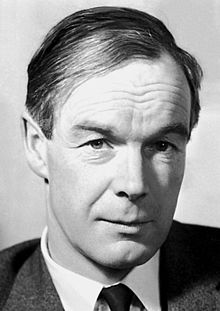
\includegraphics[height=5cm, keepaspectratio]{img/theory/hodgkin.jpg}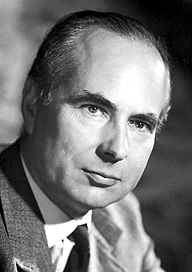
\includegraphics[height=5cm, keepaspectratio]{img/theory/huxley.jpg}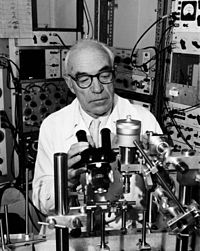
\includegraphics[height=5cm, keepaspectratio]{img/theory/eccles.jpg}
\caption[The pioneers of electrophysiology, the first to use microelectrodes.]{\emph{Sir Alan Loyd Hodgkin}, \emph{Sir Andrew Huxley} and \emph{Sir John Eccles}, the pioneers of electrophysiology, first to use microelectrodes.}
\label{fig:pioneers}
\end{figure}

They have found that the best subject for electroneurophysiological studies is the giant squid axon.
The large diameter of the axon provided a great experimental advantage for Hodgkin and Huxley; this species has large enough axons to allow the intracellular insertion of voltage clamp electrodes.
But as Graham and Gerard writes \cite{graham1946judith}:

\begin{quote}
\vspace{0.5cm}
\emph{,,The giant fiber, up to a millimeter in diameter is admirable for internal exploration with a microelectrode, since this can be inserted longitudinally and the tip pushed far from the region of penetration and damage.
These fibers are available, however, only at restricted seasons and localities and after painstaking preparation.''}
\vspace{0.5cm}
\end{quote}

Interestingly, the Second World War might have accelerated the miniaturization of the microelectrodes, because it restricted the availability of the giant squid.
Webb and Young wrote in their 1940 paper \cite{webb1940electrolyte}:

\begin{quote}
\vspace{0.5cm}
\emph{,,Unfortunately the work was terminated by the outbreak of war, which rendered the capture of further squids impossible, so that the number of fibres dealt with is much smaller than might have been wished.''}
\vspace{0.5cm}
\end{quote} 

Another species, the much more accessible longfin inshore squid (\emph{Loligo paelii}) had to be used, which has much smaller axons.
In order to carry out voltage clamp experiments on neurons of this species, the intracellular microelectrodes had to be miniaturized further.

The basic experimental setup for an early neurophysiological study employed several electrodes.
To measure the potential difference across the cell membrane, an intra- and an extracellular electrode is necessary.
This technique has been used to measure the resting potential in the axon of the squid \cite{curtis1940membrane, curtis1942membrane}.
A microelectrode consisting of a long glass capillary was pushed into one end of the axon until it reached a distance of $10-30~$mm.
To avoid causing damage to the cell membrane, great care had to be taken during this step.
The small diameter of most nerve and muscle fibres made it extremely difficult to use this technique.
The breakthrough came when Graham and Gerard showed that a very small electrode can be inserted perpendicularly into a muscle fiber without causing damage or unintentional excitation \cite{graham1946judith, ling1949normal}.
But, in order to obtain successful results, the microelectrodes should have had an external diameter of less then 0.5 $\upmu$m.
Such a small electrode diameter however introduced additional difficulties associated to the inevitable increase in electric resistance.
From that point on, the further development of microelectrodes depended on the development of the recording apparatus, as its properties combined with those of the microelectrode together determine the response characteristics.
At that time, the state of the art amplifiers were of valve types.
A few years later, advances in electronics and the technique in general made it possible to record both action, and resting potentials with these kind of electrodes \cite{hodgkin1949membrane, nastuk1950electrical}.

In 1950, Ling and Gerard published their findings in \emph{Nature} about the dependence of resting membrane potential on external potassium ion concentration \cite{ling1950external}.
The resulting plot resembled the calibration plots of ion-selective electrodes that will come a few years later.

The next big advancement in the development of microelectrodes was the introduction of the so-called \emph{patch-clamp} technique by \emph{Erwin Neher} and \emph{Bert Sakmann} \cite{neher1976single, neher1978extracellular}.
They received their Nobel Prize in 1991 \emph{,,for their discoveries concerning the function of single ion channels in cells''}, also in Physiology and Medicine.
With this technique, single ion channels were possible to observe.
The problem that had to be solved in order to be able to conduct these experiments was the large background noise.
Eher and Sakmann wrote in their original Nature paper \cite{neher1976single}:

\begin{quote}
\vspace{0.5cm}
\emph{,,Clearly, it would be of great interest to refine techniques of conductance measurement in order to resolve discrete changes in conductance which are expected to occur when single channels open or close.
This has not been possible so far because of excessive extraneous background noise.''}
\vspace{0.5cm}
\end{quote} 

To solve this problem, they measured transmembrane ionic current only on a small, isolated area of the cell membrane.
This was achieved by pushing the tip of a $d_o = 3-5~\upmu$m glass micropipette onto the cell membrane, and limiting the measurement to a small patch of the membrane, ideally featuring only a single ion channel.
By measuring the current in this way, the two states of a single ion channel -- closed and open -- were possible to distinguish.
Eher and Sakmann were able to detect the discrete conductance changes of the ion channel associated to the acethylcholine receptor in the neuromuscular junction. 

\subsection{Glass-based electrodes and microelectrodes}
Analytical potentiometry started with the discovery and development of the glass pH-electrode. It is the best electrochemical sensor, and one of the best sensor ever made, with a linear response over more than 13 orders of magnitude, and excellent selectivity.
Because of its importance, and because pH measurement is used throughout the work described in this thesis, the basic concepts of pH measurement will be introduced through the example of the glass electrode.

It was in 1906, when a botanist named Max Cremer discovered that the potential difference across a thin glass membrane is a function of pH when opposite sides of the membrane are in contact with solutions containing different concentrations of H$_3$O$^+$ \cite{cremer1906ursache, cremer1906direkte}.
Three years later, in 1909, S\o rensen introduced the concept of pH \cite{sorensen1909messung}.
He defined it as the negative logarithm of the concentration of H$_3$O$^+$:

\begin{equation}
\textrm{pH} = -\lg c_{\textrm{H}_3\textrm{O}^+}
\end{equation}

This however, is not entirely true, because pH depends on the \emph{activity} of H$_3$O$^+$, rather than its concentration:

\begin{equation}
\textrm{pH} = -\lg a_{\textrm{H}_3\textrm{O}^+}
\end{equation}

And since pH is dimensionless, a better way to define pH is:

\begin{equation}
\textrm{pH} = -\lg(\gamma_{\textrm{H}_3\textrm{O}^+} m_{\textrm{H}_3\textrm{O}^+} / m^\theta)
\end{equation}

or

\begin{equation}
\textrm{pH} = -\lg(\gamma_{\textrm{H}_3\textrm{O}^+} c_{\textrm{H}_3\textrm{O}^+} / c^\theta)
\end{equation}

where $m^\theta$ = 1 mol$\cdot$kg$^{-1}$ and $c^\theta$ = 1 mol$\cdot$dm$^{-3}$ are the standard states, and $\gamma_{\textrm{H}_3\textrm{O}^+}$ is the activity coefficient of H$_3$O$^+$. 

The current, internationally accepted definition of pH is an instrumental definition, based on an electrochemical cell known as the \emph{Harned Cell} \cite{harned1958activity} (Fig. \ref{fig:harned}).
To measure the pH in such a cell, a conventional procedure was developed at NBS (National Bureau of Standards) \cite{durst1975standardization} and recommended at present by the last IUPAC (International Union of Pure and Applied Chemistry) Recommendations \cite{covington2002measurement}.
NIST (National Institute of Standards and Technology) in the U.S. and PTB (Physikalisch-Technische Bundesanstalt) in Germany have presented pH values using the Harned Cell. 

\begin{SCfigure}
\centering
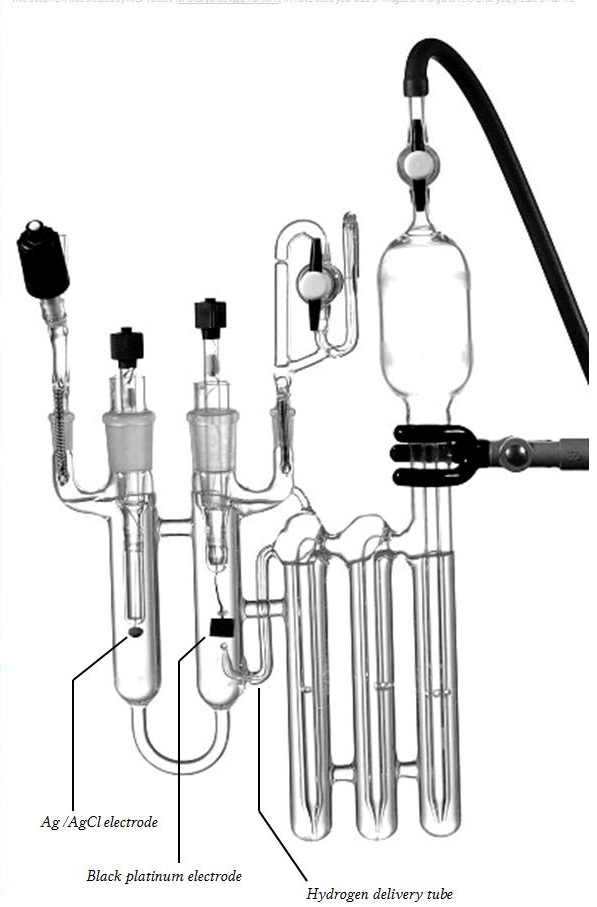
\includegraphics[height=10cm, keepaspectratio]{img/theory/Harned_bw.jpg}
\caption{The Gold Standard of pH measurement, the Harned cell (at the Danish National Metrology Institute).}
\label{fig:harned}
\end{SCfigure}

The Harned Cell is described by the following cell diagram: 

\begin{equation}
\textrm{Pt(s) | H}_2\textrm{(g) | buffer solution, Cl}^-\textrm{(aq) | AgCl(s) | Ag(s)}
\label{eq:harned}
\end{equation}

To calculate the potential of the half-cells, the \emph{Nernst-equation} can be used:

\begin{equation}
E = E^\theta - \frac{RT}{z_iF}\ln a_i
\end{equation}

where $E^\theta$ is the standard potential difference of the cell, $R$ the universal gas constant, $F$ the Faraday constant, $T$ the thermodynamic temperature, $z_i$ is the valence and $a_i$ is the activity of ion species $i$.
The potential difference $E$ of the cell \ref{eq:harned} is described by the \emph{Nernst-equation} as:

\begin{equation}
E = E^\theta - \frac{RT\ln 10}{F}\lg\bigg(\frac{a_{\textrm{H}_3\textrm{O}^+}m_{\textrm{Cl}^-}\gamma_{\textrm{Cl}^-}}{m^\theta}\bigg)
\end{equation}

After expressing the pH:

\begin{equation}
\textrm{p}(a_{\textrm{H}_3\textrm{O}^+}\gamma_{\textrm{Cl}^-}) = -\lg(a_{\textrm{H}_3\textrm{O}^+}\gamma_{\textrm{Cl}^-}) = \frac{E - E^\theta}{(RT/F)\ln10} + \lg \bigg(\frac{m_{\textrm{Cl}^-}}{m^\theta}\bigg)
\end{equation}

where $\gamma_{\textrm{Cl}^-}$ is the molal activity coefficient of the chloride ions at the molality $m_{\textrm{Cl}^-}$.

By extrapolating on the equation obtained with least square fitting, the value of the acidity function at zero chloride ion molality p$a_0$ = $-$lg($a_{\textrm{H}^+} \gamma _{\textrm{Cl}^-})m_{\textrm{Cl}^- \to 0}$ can be determined.
Applying the Bates -- Guggenheim convention \cite{bates1960report}, the trace activity coefficient of chloride ions $\gamma_{\textrm{Cl}^- \to 0}$ at $m_{\textrm{Cl}^- \to 0}$ can be calculated:

\begin{equation}
\lg \gamma_{\textrm{Cl}^- \to 0} = \frac{A I^{1/2}}{1 + 1.5I^{1/2}}
\end{equation}

where $A$ is the Debye-Hückel temperature-dependent limiting slope and $I$ the ionic strength of the buffer solution calculated by $I = (1/2) \Sigma c_i z_{i}^{2}$, where $c_i$ and $z_i$ are the molar concentration and electric charge of ionic species $i$.

Haber and Klemensiewicz gave a full account of the response of the glass electrode in their 1909 paper \cite{haber1909elektrische, haber1909concerning}.
The next advance towards the microelectrodes was the miniaturization of the glass electrode by Caldwell in 1954 \cite{caldwell1954investigation}.
He used it to measure intracellular pH in crab muscle fibers.
Hinke created ion-selective electrodes for potassium and sodium using the respective sensitive glasses developed by Eisenmann, Rudin and Casby two years earlier \cite{eisenman1957glass}, based on the work of Lengyel \cite{lengyel1934behaviour} published in 1934.
He used them to show the correlation between sodium ion concentration in blood, and blood pressure \cite{friedman1958use, friedman1959drug}.
Also, similarly to what Caldwell did with the glass electrode, Hinke created sodium and potassium ion-selective microelectrodes in 1959 \cite{hinke1959glass} using the same type of ion selective glasses.
With his revolutionary \textbf{\emph{ion-selective microelectrodes}} (Fig. \ref{fig:hinke}), Hinke was able to perform the first true intracellular ion-selective measurements, and determined the potassium and sodium ion concentration in the muscle cells of the propodite of crab and lobster (\emph{Carcinus m\ae nus} and \emph{Homarus vulgaris}).
His microelectrodes originally had a tip cross section of 20 $\upmu$m $\times$ 150 $\upmu$m, with a wall thickness of 1 -- 4 $\upmu$m, and a resistance of $10^{10} - 10^{11}$ $\ohm$.

\begin{SCfigure}
\centering
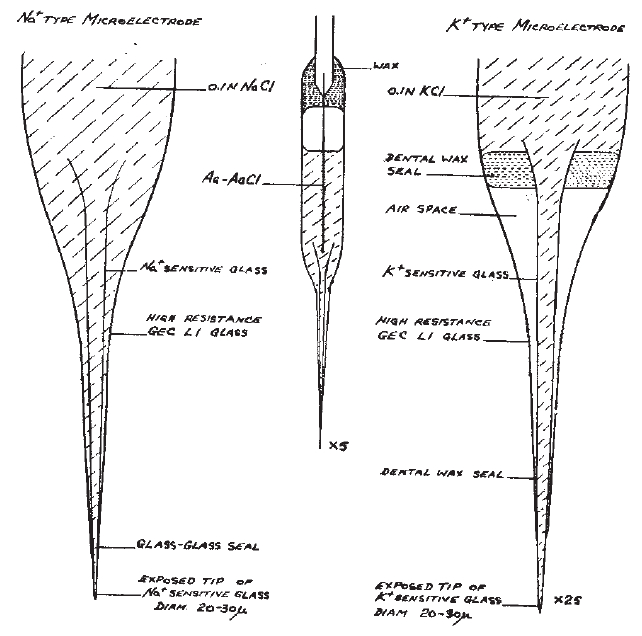
\includegraphics[height=9cm, keepaspectratio]{img/theory/hinke.jpg}
\caption[The first true ion-selective microelectrodes, created by Hinke.]{The first true ion-selective microelectrodes, created by Hinke to measure intracellular sodium, and potassium ion concentration.
As published in his 1959 \emph{Nature} paper \cite{hinke1959glass}.}
\label{fig:hinke}
\end{SCfigure}

\subsection{Liquid ion exchanger membrane based microelectrodes}
While Hinke was able to eventually decrease the tip diameter of his ion-selective microelectrodes to 1 $\upmu$m or less, the sensitive area was too large ($\sim 10~\upmu$m in length, and $\geq5~\upmu$m in diameter).
In order to measure intracellular ion activity, it was necessary to push the entire sensitive part into the cell, causing significant damage.
In addition to the problem of size, they were difficult to fabricate.

By that time, liquid ion exchangers have been used in liquid-liquid ion extraction processes in industry and, and as models for biological membranes \cite{beutner1913new, eisenman1967membrane}.
Sandblom, Eisenmann and Walker published two papers in 1971 about a rather exhaustive theoretical treatment of such liquid ion exchanger (LIX) membranes \cite{walkerLIX1, walkerLIX2}.
Also in 1971, Walker was able to prepare a miniaturized version of the electrodes based on the LIX membranes \cite{walker1971ion}.
He writes in \cite{walker1971ion}:

\begin{quote}
\vspace{0.5cm}
\emph{,,A liquid ion exchanger is composed of an organic electrolyte dissolved in a water-immiscible solvent, usually an organic solvent with a low dielectric constant.
Owing to the low dielectric constant of the exchanger, inorganic ions have a very low solubility in the exchanger and, consequently, a membrane made of a liquid ion exchanger is much more permeable to ions whose valence sign is opposite to that of the organic ion than to ions of the same valence sign because of ion pair formation with the organic ion.''}
\vspace{0.5cm}
\end{quote} 

\label{silanize}
Walker also added a crucial step to the fabrication of these microelectrodes: the silanization of the inner surface of micropipette.
The surface of the glass pipette is highly hydrophilic owing to the silanol groups, and the sensing membrane in the pipette tip is hydrophobic.
To improve the adhesion of the two, and to prevent the electrolyte from creeping along the pipette wall from either side, Walker silanized the surface.
This step improved stability and life-time of these microelectrodes drastically.

He used the new LIX ion-selective microelectrodes to measure chloride, and potassium ion activity in \emph{Aplysia} neurons.
He estimated the resistance for his electrodes from their response time in the range of $10^9$ to $10^{10}$ $\ohm$.
He also performed selectivity measurements on the microelectrode, using the Nicolsky-equation \cite{nicolsky1937theory}:

\begin{equation}
E=E^\theta + \frac{RT}{z_iF} \ln \left [ a_i + \sum_{j} \left ( k_{ij}a_j^{z_i/z_j} \right ) \right ]
\end{equation}

where $E$ is the open circuit potential, $E^\theta$ the standard electrode potential, $z$ and $a$ are the valency and the activity of the ionic species $i$ and $j$. k$_{ij}$ is the selectivity coefficient with respect to $j$.
These microelectrodes were surpassed by the following generation of ion-selective microelectrodes, based on the ionophores.

\subsection{Ionophore based microelectrodes}
\label{ionophore_based}
The ion-selective microelectrodes used today are based on the ionophores.
These are carriers for specific ions, and act as complexing ligands.
\v{S}tefanac and Simon published their work concerning the use of nonactin, a lipophilic antibiotic, as ionophore in ion-selective membranes \cite{stefanac1966highly, vstefanac1967ion}.
Their cell consisted of the following elements:

\begin{equation}
\text{Ag | AgCl | KCl(aq) || membrane || sample | NH$_4$NO$_3$(aq) | KCl(aq) | Hg$_2$Cl$_2$| Hg}
\end{equation}

They dissolved nonactin and nonactin homologs in carbon tetrachloride, and transferred onto sintered glass discs to form a membrane.
Their cell showed a selectivity for certain cations, especially potassium and ammonium ions \cite{stefanac1966highly, vstefanac1967ion}. 

For quite some time after the discovery that ionophores can be used in ion selective electrodes, the LIX membrane based ion selective microelectrodes were used instead.
The reason for this is the relatively high resistance of the membranes employing the neutral carrier ionophores.
They had however, a great adventage over the LIX membranes: their selectivity.
In cases, as Amman writes in his 1987 paper \cite{ammann1987valinomycin} it reached a factor of 5000:

\begin{quote}
\vspace{0.5cm}
\emph{,,[With the valinomycin based microelectrodes ... ] extremely high K$^+$ selectivities are obtained, e.g. a rejection of Na$^+$ by a factor of 5000 and of acetylcholine by a factor of 3400.
At a constant background of 140 and 500 mM Na$^+$, the detection limit of the K$^+$ sensor is at $1.6\times  10^{-5}$ and at $2.5\times 10^{-5}$ M K$^+$, respectively.''}
\vspace{0.5cm}
\end{quote}

and 

\begin{quote}
\vspace{0.5cm}
\emph{,,Valinomycin-based microelectrodes will find increasing application only if their electrical resistances can be further reduced without inducing a loss in} K\emph{$^+$ selectivity.''}
\vspace{0.5cm}
\end{quote}

Oehme and Simon did a comparison of the two types much earlier, in 1976 \cite{oehme1976microelectrode}, and already realized the major difference between the two.
A slightly improved version by Wuhrmann \cite{wuhrmann1979change} found only limited use in physiology.
In both of these papers, valinomycin based microelectrodes with a very high resistance (R = $10^{11}\; \ohm$) are described.
Such high resistances of course result in very long response times ($\tau > 30~s$). 

The big breakthrough came when Ammann realized, that the resistance of neutral carrier-based membranes can be lowered drastically if both lipophilic salts and polar membrane solvents are added to the membrane \cite{ammann1987valinomycin}.
With this improvement, he lowered the resistance and essentially got the same as the LIX membranes had at the time, but managed to maintain the extremely high selectivity.

\begin{figure}[h]
\centering
A 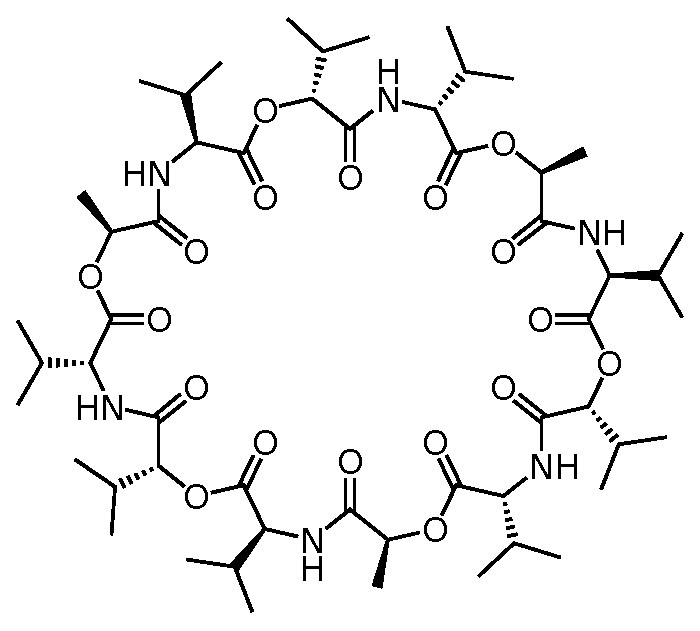
\includegraphics[width=0.4\textwidth]{img/theory/Valinomycin.eps}\hspace{1cm} B 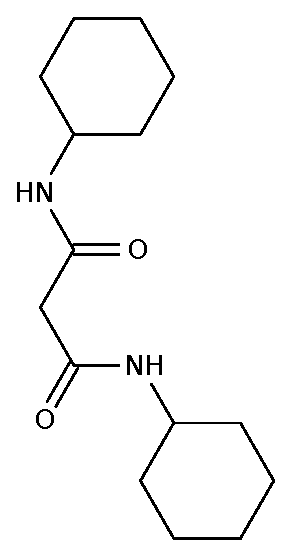
\includegraphics[width=0.18\textwidth]{img/theory/mg_ionophore.eps}

\vspace{1cm}

C 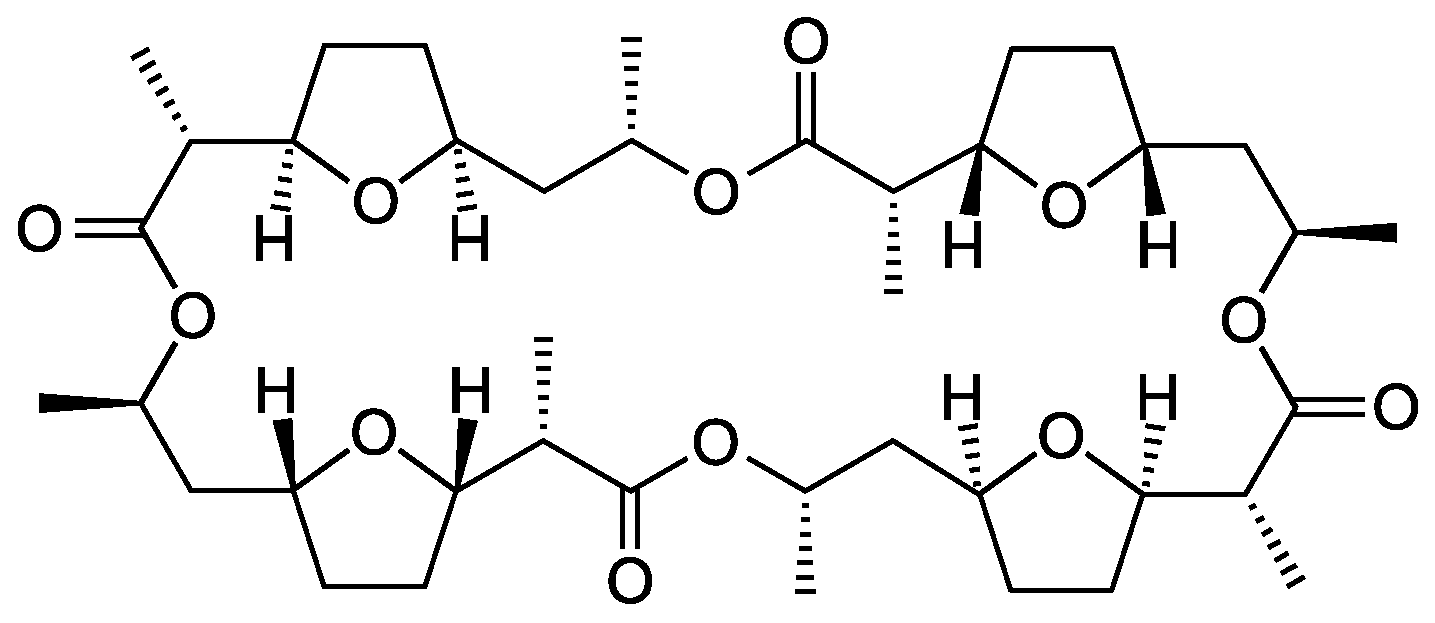
\includegraphics[width=0.5\textwidth]{img/theory/Nonactin.eps}
\caption{(A) Valinomycin, (B) bis-N,N-dicyclohexyl-malonamide, and (C) nonactin, ionophores for potassium, magnesium, and ammonium ions, respectively.}
\label{fig:ionophores}
\end{figure}

The first synthesized ionophores were introduced in 1969 by Kimura and co-workers \cite{kimura1979potassium}.
Since then, many research groups synthesized ionophores for many different ions.

pH and blood gases have been measured routinely since Severinghaus and Bradley developed the blood gas analyzer for CO$_2$ and O$_2$ in 1958 \cite{severinghaus1958electrodes}.
These are not based on ionophores, but will be described here briefly because they are related closely to the metal/metal-oxide microelectrodes used in this dissertation.
To measure oxygen, they used Clarks electrode \cite{clark1953continuous}, and for carbon-dioxide, they developed a gas gas sensor, which since has been known as the \emph{,,Severinghaus--electrode''}.
It is based on pH measurement in a thin membrane on the surface of a glass pH-electrode.
Carbon-dioxide diffuses to the membrane, dissolves in the thin film, and lowers the pH.
The cell has been miniaturized by several research groups \cite{cai1993development, de1997fast, zhao1997improved, hanstein2001miniaturised, beyenal2004improved}.
The cited papers are all using an improved, miniaturized, microelectrode version of the original electrode.
I used a similar, antimony based miniaturized Severinghaus--electrode in my masters thesis \cite{msc2011}, and published spatially resolved CO$_2$ measurements -- with the same electrode -- of living yeast colonies in \cite{kiss2011air}.

A big advancement in the field of ion-selective electrodes was the elimination of the internal filling solution from the conventional ion-selective electrodes.
This resulted in the so-called \emph{solid-contact} electrodes.
The first of these were unstable, because there was no reversible and fast ion-to-electron transducer \cite{nikolskii1985solid}.
Solid-contact electrodes had already been around since the 1970s with the invention of the coated-wire electrode (CWE) \cite{cattrall1971coated}.
The instability was solved by the electropolymerization of a thin layer of conductive polymer onto the solid contact, that showed a mixed electronic and ionic conductivity, thereby providing a stable ion-to-electron interface \cite{bobacka2003potentiometric, bobacka2004all, bobacka2006conducting, michalska2006optimizing}.
A wide range of conductive polymers are used, including polypyrroles \cite{sun2004construction}, polythiophenes \cite{bobacka1994all}, and polyanilins \cite{paciorek2005miniature}.
In this thesis, the ion-to-electron interface in the solid-contact ion-selective microelectrodes is PEDOT (poly(3,4-ethylenedioxythiophene)), first used for this purpose by Johan Bobacka and coworkers \cite{bobacka1994all}.
Solid-contact electrodes were used in the work done in our laboratory earlier \cite{gyetvai2007solid, varga2011development, izquierdo2012scanning}.

An interesting application of solid-contact microelectrodes is described in \cite{kounaves2002determination}.
An array of electrochemical sensors, including 27 microlectrodes were used to determine the concentration of certain ions in the martian soil.
This is a good demonstration of how little and simple instrumentation is enough to carry out potentiometric measurements.
During Mars missions it is extremely important that the carried instruments are reliable, robust, and light.
The reason behind the choice of microelectrodes in this case wasn't based solely on the scale of the measurement -- the solvent had to be carried to Mars by the vessel in its ,,wet chemistry cells'' --, but also the mass of the payload carried by the vessel.

The ,,golden age'' of ion selective microelectrodes was certainly during the period of $1960-1980$.
One of the most prominent research groups in that time was lead by professor Ernő Pungor.
After this period the next big advancement in the field came at the end of the 1990s by better understanding the theory behind the ion selective microelectrodes, and a consequent lowering of their lower detection limit.
The lower limit of detection of ion-selective electrodes has usually not been lower than $10^{-6}$ M.
Several research groups have achieved better results recently by optimizations \cite{sodergaard2003lowering}.
By carefully choosing the measurement parameters to reduce side reactions and parasitic processes such as the influence of interferring ions, subnanomolar lower detection limits can be achieved \cite{lisak2010study}.
In \cite{lisak2011tuned} the authors describe a method called tuned galvanostatic polarization, which successfully facilitates the membrane to work in less oxidizing conditions, thereby reducing the lower detection limit.
Lower limit can be achieved by drastically reducing zero-current ion fluxes from the membrane in the direction of the sample \cite{malon2006potentiometry}.
Such ion fluxes have notoriously prevented achieving better detection limits and selectivities with such sensors \cite{sutter2004solid}.
The lower detection limit is an important parameter of potentiometric ion-selective microelectrodes.
Every success in this respect advances their usability greatly.
There are many advantages of the potentiometric ion-selective electrodes, such as their simplicity, their relative speed compared to other methods and the great potential for their miniaturization.
One area where they are certainly behind most analytical methods is their lower detection limit.
Recently, advances have been made in this area as well, thanks to the more and more sophisticated theoretical descriptions of such electrodes \cite{jasielec2010comparison}.

The above mentioned models are improvements over the previous, Phase Boundary Model (PBM).
This model is assuming local equilibrium between the adjacent phases (aqueous/organic/aqueous) -- and therefore throughout the whole system.
Equilibrium in charged systems regarding an ion is realized when the electrochemical potential of that ion in the phases of the system is equal. The electrochemical potential of a phase can be given by the equation that was first introduced by Guggenheim \cite{guggenheim1929conceptions, guggenheim1930conception}:

\begin{equation}
\bar\mu_i = \mu_i + z_i F \phi = \mu_i^0 + RT\ln a_i + z_i F \phi
\end{equation}
where $\phi$ is the Galvani potential.
The PB model neglects any kinetic parameter, for instance the mobilities of ions.
The model is summarized by the following equation:

\begin{equation}
E_{PB} = \frac{RT}{z_i F}\ln k_i + \frac{RT}{z_i F}\ln \frac{a_i(aq)}{a_i(org)}
\end{equation}
where $a_i(aq)$ and $a_i(org)$ are the activity of ion $i$ in the aqueous and the organic phase, $z_i$ is its charge. $k_i$ is a function of the relative free energies of solvation in both the sample and the membrane phase \cite{bakker2004phase}.

To account for the influence of kinetic parameters in a wide range of phenomena involving charged particles -- including the behaviour of ion selective electrodes --, the Nernst -- Planck -- Poisson (NPP) model \cite{planck1890ueber, nernst1889elektromotorische, planck1890ueber2} can be used.
This model successfully accounts for several parameters of ion selective electrodes, including their selectivity \cite{lingenfelter2006time} and lower detection limit \cite{sokalski2009time}.
The model has recently been adopted for the theoretical description of ion selective electrodes employing neutral ionophores by Lewenstam et al. \cite{jasielec2015neutral}.
The description therein is an improvement of the NPP model.
Besides the transport of ion $i^+$ between the three phases:

\label{ligand}

\begin{equation}
  i^+_{sample} \ce{<=>} i^+_{membrane} \ce{<=>} i^+_{inner  solution}
\end{equation}

the reaction between the measured ion and the ligand -- complexing the ion -- is considered as well:

\begin{equation}
  i^+_{membrane} + L_{membrane} \ce{<=>} iL^+_{membrane}
  \label{eq:ligand_reaction}
\end{equation}

Previously this reaction has been regarded infinitely fast.
However by considering this process, a more accurate model can be obtained.
The rate of this reaction can be an additional factor determining the response characteristics of an ion selective microelectrode.

\subsection{Metal/metal-oxide pH microelectrodes}
Since the glass electrode cannot be effectively miniaturized due to the reasons detailed in the previous sections, intensive research has been conducted for several decades to improve metal/metal-oxide electrodes.
One of the most often used type of these is the Ir/IrO$_2$ electrode \cite{beyenal2004improved}.
The oldest is certainly the Sb/Sb$_2$O$_3$ electrode, its initial characterization dating back to 1923 \cite{uhl1923electrometric}.
It is based on the equilibrium between antimony and the antimony-oxide on its surface.
It is pH sensitive because hydrogen ions participate in the equilibrium:

\begin{equation}
        \ce{2Sb_{(s)} + 3H_2O <=> Sb_2O_3 + 6H^+ + 6e^-}
\end{equation}

\begin{equation}
        \ce{Sb_{(s)} + 3OH^- <=> Sb(OH)_3 + 6e^-}
\end{equation}

Using the Nernst-equation to describe the relationship between [Sb$^{3+}$] and the measured electrode potential \cite{kurzweil2009metal}:

\begin{equation}
E = E^\theta - \frac{RT}{3F}\ln a_{\textrm{Sb}^{3+}}
\end{equation}

Which can be rewritten by using $K_W$, the water ion product, and $K_L$, the solubility product of antimony hydroxide as \cite{kurzweil2009metal}:

\begin{equation}
E = E^\theta - \frac{RT}{3F}\ln \frac{K_L}{K_W} + \frac{RT}{F}\ln a_{\textrm{H}^+}
= E^{\theta '} - \frac{RT}{0.4343F} \textrm{pH}  
\end{equation}
because [Sb$^{3+}$]=[H$^+$]$\cdot K_L / K_W$.

The main reason this particular electrode is so popular is that the melting point of antimony and the softening point of borosilicate glass are similar ($T_{m, \textrm{Sb}} = 630.63~\celsius$, $T_{m, glass}\approx 700~\celsius$), and manufacturing them is relatively easy with standard glass blowing techniques.

Another very popular metal/metal-oxide electrode used for pH measurements is the tungsten electrode. Its function is also based on the equilibrium between the metal and its oxide:
\begin{equation}
        \ce{W_{(s)} + 3H_2O <=> WO_3 + 6H^+ + 6e^-}
\end{equation}

Although semiconductor based microsensors differ in how they work, I would like to mention the ISFETs (Ion-Selective Field-Effect Transistor) here.
They can be used to measure ion concentration, originally developed to measure H$^+$.
The solution is the \emph{,,gate''} electrode, and the conductivity between the \emph{,,source''} and the \emph{,,drain''} terminals depends on the ion activity in the solution adjacent to the gate.
The technique was invented by Piet Bergveld in 1970 \cite{toumazou2011piet}.


		\subsection{The potentiometric measurement}
The generation and measurement of the voltage in the potentiometric cell are closely related.
Unfortunalety, as with any other technique, the measurement itself influences the investigated system, and therefore the measured value.
This effect is especially strong in potentiometry.
Fig. \ref{fig:loading_error} shows the circuit diagram of the generation and measurement of the voltage.
First it will be discussed as if the amplifier wasn't present in the circuit.
Without the amplifier, it can be split into three parts \cite{halliwell1987using}:

\begin{figure}
\centering
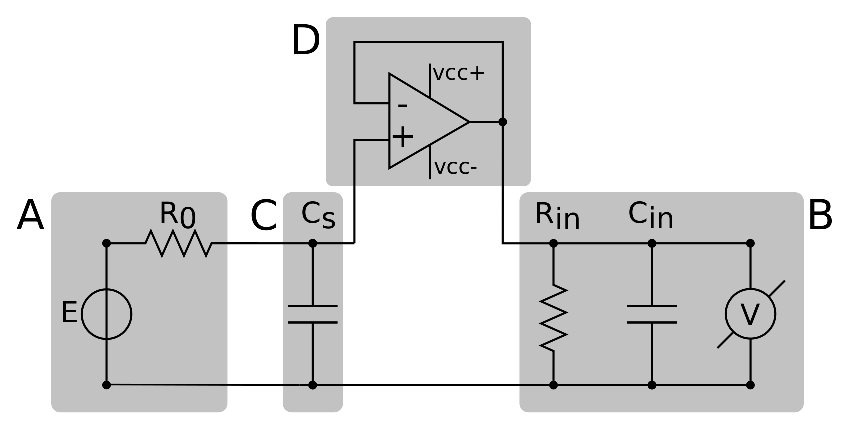
\includegraphics[width=0.7\textwidth]{img/theory/loading_error_2.eps}
\caption[The model of the potentiometric measurement.]{The model of the potentiometric measurement. The circuit is constituted by 4 parts: (A) voltage source, the potential difference between the reference and the measuring electrodes with an $R_0$ output resistance. (B) The measuring circuit, which can be split into 3 elements: a voltmeter, a resistance $R_{in}$ to account for current flowing through the terminals of the voltmeter, and an input capacitance $C_{in}$. (C) The electrical connection between the voltage generator and the measuring circuit, with a capacitance $C_s$. (D) Unity gain current buffer built from an operational amplifier in the non-inverting voltage follower configuration.}
\label{fig:loading_error}
\end{figure}

\emph{(A) Source of the voltage}.
The potential difference $V$ is developed across the output of an ideal voltage source $E$ in series with a large output resistance $R_0$.
In the potentiometric cell, $R_0$ is the resistance of the measuring electrode, and $E$ is the potential of the measuring electrode with respect to the reference electrode.
Although $E$ is regarded perfect in this model, and its voltage is independent of the current drawn, the output voltage $V$ is smaller than $E$, because of the ohmic drop $iR_0 = E - V$.
Since the resistance of a microelectrode can be in the range of mega-, or even gigaohms, very large errors may result from very small currents.

\emph{(B) The measuring circuit} consist of three elements.
The first element is the voltmeter $V$ with infinitely large input impedance. It draws no current, since $i = U/\infty=0$. It doesn't have any input capacitance ($C_{in}$ is modeled separately), therefore it responds to the input voltage without any delay.
The second element is a resistance $R_{in}$ to account for the imperfection of real voltmeters, the current flowing through its terminals as a consequence of the potential difference between them.
The third element is the input capacitance of the voltmeter, modeled by the capacitor $C_{in}$.
The current flowing through $R_{in}$ is $i_{R_{in}}=V/R_{in}$. It equals to the difference between the input and the output of the circuit, the error of the measurement of $E$:

\begin{equation}
\label{eq:loading}
	E - V = i_{R_{in}} R_0 = \frac{R_0 V}{R_{in}}
\end{equation}

The ratio of the two can be calculated by the formula for the voltage divider: 

\begin{equation}
\label{eq:loading2}
        \frac{V}{E} = \frac{R_{in}}{R_0+R_{in}}
\end{equation}

Input resistance $R_{in}$ of a typical voltmeter is in the range of $1-10$ M$\ohm$.
This relatively low resistance can cause a large distortion, because $R_{in}/(R_0+R_{in})$ approaches 1 only if $R_{in}$ approaches infinity, or $R_0$ approaches zero.
Since $R_0$ is a given property of the circuit, the only way the error can be lowered is by increasing $R_{in}$.
For example, the input resistance of a microelectrode amplifier is about $10^{12}$ $\ohm$, and of a pH meter $\sim 10^{14}$ $\ohm$.
Based on Eq. \ref{eq:loading} it is very important that $R_{in} \gg R_o$ to minimize the error in potential measurements.
The effect of input capacitance $C_{in}$ is discussed in the next section (\emph{Response characteristics}).

\emph{(C) The connection} between the voltage source $E$ and the measuring instrument $V$.
This element influences the measurement in two ways.
First, it delays the voltage across $V$ compared to $E$, the effect which is detailed in the next section (\emph{Response characteristics}).
The other effect is a consequence of a very small current, induced by stray capacitance.
The cable between $E$ and $V$ acts as the plate of a capacitor.
The other plate can be anything in the environment.
If the capacitance of the element constituted by these two plates changes -- by objects moving around in the environment, or charge transfer occuring -- small current will flow through the cable.
Since the overall resistance of the circuit is quite high due to the measuring microelectrode, even if very small currents are induced by the stray capacitance, large amount of noise can be added to $V$, because $V = iR_0$.
This effect can be minimised by using shielded cables to decrease stray capacitance, and using as short connections between the high impedance elements and the amplifier as possible.
Stray capacitance of a typical shielded (braided) cable is $\sim 100-200~$pF/m.

\emph{(D) Operational amplifiers} are used to solve several of the issues described above.
They are introduced between the measuring electrode and the measuring circuit as seen in Fig. \ref{fig:loading_error}.
The operational amplifier is used as a \emph{unity gain current buffer}.
It is achieved by connecting the output of the amplifier to the inverting input.
In this configuration, the output is tied back to the inverting input, while the potential to be measured (with respect to ground) is connected to the non-inverting input.
Since the operational amplifier does everything it can to keep the two inputs at the same voltage, and one of the output is fed back to one of the inputs, the output will be the same as the other input.  
The name of this circuit is \emph{non-inverting voltage follower}.
It comes from the fact that the output $V_{out}$ follows $V_{in}$, and the sign of the two equal, as opposed to the inverting configuration, when $V_{out}=-V_{in}$.
In other words, the circuit has unity ($\times 1$) gain: it does not amplify potential difference.
The reason this circuit is used as an interface between the high impedance source and the low impedance measuring circuit is that because of its high input impedance, it draws no current from the source.
Therefore there is no loading error on its high impedance side.
On the other hand, they have a low output impedance, and can drive the measuring instrument, with minimal $R_0$ of their own, and therefore there is no loading error on the low impedance side either.
The input impedance of a typical opamp used for this purpose is around 1$-$10 T$\ohm$, so $R_{in}/(R_{in}+R_0)$ is unity, and the measured $V$ is almost identical to the source $E$, because $V/E$ is also 1.

		\subsection{Response characteristics}
\subsubsection{Possible contributors determining the potentiometric response}
There are several steps constituting the potentiometric response that can be responsible for a delay:

\begin{enumerate}
\item Transport of the measured ion to the sensitive surface.
\item Flux of the measured ion through the phase boundary.
\item Complexation reaction between the measured ion and its ligand.
\item RC delay.
\end{enumerate}

Usually the consequence of only one of these can be observed in the response of a particular type of electrode. That is because that one process -- called the \emph{rate determining step} -- is much slower than the rest. Figure \ref{fig:rds}. illustrates steps 1--3.
\begin{figure}[t]
\centering
\includegraphics[width=0.7\textwidth]{img/rds.eps}
\caption[The possible contributors to the delayed response of the potentiometric cell.]{The possible contributors to the delayed response of the potentiometric cell. (1) Transport of the measured ion to the sensitive surface. (2) Flux of the measured ion through the phase boundary. (3) Complexation reaction between the measured ion and its ligand.}
\label{fig:rds}
\end{figure}
During the first step, the measured ion has to be transported to the phase boundary. Depending on whether there is stirring or not, this can either be realized by convection and diffusion, or diffusion alone. In cases where this step is the rate determining, stirring should decrease the response time of the cell.

In the second step, the ion has to cross the phase boundary between the sample solution and the ion-selective membrane. The lower the activity of the measured ion in the sample, the lower this flux will be. In the case of an ion-selective micropipette employing a neutral ionophore, the next step is the complexation reaction between the ion and the ligand. This step has already been mentioned previously in section \ref{ligand}, more specifically by Eq. \ref{eq:ligand_reaction}. If the concentration in the membrane is constant, the this reaction can be regarded a first order reaction, and as such its behaviour can be described by the function $e^{-kt}$, $k$ being the rate constant.

And finally, there is an RC delay associated with the potentiometric cell, described in the next section.

\subsubsection{RC delay}
In this section the response delay associated with the $RC$ time constant is considered.
Because the $RC$ time-constant plays a central role in my thesis, I give a detailed derivation of it here.
The potentiometric cell can be modeled as a series $RC$ circuit (Fig. \ref{fig:rc}).
Kirchhoff's second law states that the directed sum of the electrical potential differences (voltages) around any closed network is zero \cite{hill2015art}:


\begin{equation}
\label{eq:kirchoff}
	\sum_{k=1}^{n} V_k = 0
\end{equation}

where $n$ is the total number of voltages measured across the loop.
This must be true for the energy to be conserved.
Using Ohm's law to express the voltage across the resistor as $iR$ and Kirchhoff's second circuit law on the series $RC$ circuit, we get:

\begin{equation}
\label{eq:loop1}
	V_{in} - iR - V_{out} = 0
\end{equation}

where $i$ is the current flowing through any two points of the circuit clockwise.
Since $i$ is nothing but the change of charge in time, $i = \mathrm{d}q / \mathrm{d}t$, and $V_{out} = q / C$, Eq. \ref{eq:loop1} can be rewritten as

\begin{equation}
\label{eq:loop2}
        V_{in} - \frac{\mathrm{d}q}{\mathrm{d}t}R - \frac{q}{C} = 0
\end{equation}

\begin{figure}
\centering
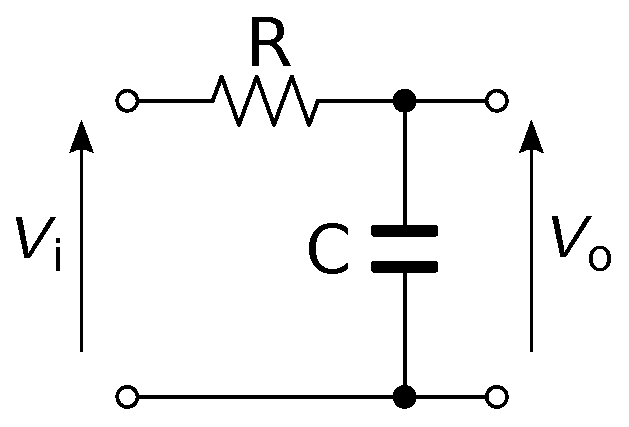
\includegraphics[width=0.4\textwidth]{img/theory/rc.eps}
\caption{The series $RC$ circuit.}
\label{fig:rc}
\end{figure}


This can be rearranged to

\begin{equation}
\label{eq:loop3}
        \frac{\mathrm{d}q}{\mathrm{d}t} = \frac{1}{R}\bigg(V_{in} - \frac{q}{C}\bigg)
\end{equation}

After cross multiplication we get

\begin{equation}
\label{eq:loop4}
        \frac{\mathrm{d}q}{V_{in}-\displaystyle{\frac{q}{C}}} = \frac{\mathrm{d}t}{R}
\end{equation}

Rearranging it leads to

\begin{equation}
\label{eq:loop5}
        \frac{\mathrm{d}q}{q - CV_{in}} = - \frac{\mathrm{d}t}{RC}
\end{equation}

To get $q$ as a function of $t$, we need to integrate.
At $t = 0$ the capacitor is not charged, so $q = 0$.
Then, as we apply the voltage $V_{in}$, the capacitor slowly starts charging, until we arrive at a charge $q$:

\begin{equation}
\label{eq:loop6}
        \int_{0}^{q} \frac{\mathrm{d}q}{q - CV_{in}} = \int_{0}^{t} - \frac{\mathrm{d}t}{RC}
\end{equation}

or

\begin{equation}
\label{eq:loop7}
        \ln(q(t) - CV_{in})\Bigr|_{0}^{q} = - \frac{t}{RC}\Bigr|_{0}^{t}
\end{equation}

After solving we get

\begin{equation}
\label{eq:loop8}
        \ln\bigg(\frac{q(t) - CV_{in}}{-CV_{in}}\bigg) = - \frac{t}{RC}
\end{equation}

If we raise both sides to the natural exponent, we get

\begin{equation}
\label{eq:loop9}
        \frac{q(t) - CV_{in}}{-CV_{in}} = e^{-t/RC}
\end{equation}

Solving for $q(t)$:

\begin{equation}
\label{eq:loop10}
        q(t) = CV_{in}(1 - e^{-t/RC})
\end{equation}

Since the voltage across the capacitor is $V_{out} = q / C$, dividing both sides by $C$ leads us to

\begin{equation}
\label{eq:loop11}
        V_{out}(t) = V_{in}(1 - e^{-t/RC})
\end{equation}

This is the general expression to the voltage across a charging capacitor at any time instance $t$.
To find the expression for the voltage when the capacitor is discharging, very much the same way we get:

\begin{equation}
\label{eq:loop12}
        V_{out}(t) = V_{in}e^{-t/RC}
\end{equation}

$RC$ is the time constant of the series $RC$ circuit, denoted as $\tau$ in general.
Observing Eqs. \ref{eq:loop11}-\ref{eq:loop12}, it is the time that it takes to charge the capacitor by 63.2\% ($1 - e^{-1} = 0.632$), or to discharge it by 36.8\% ($e^{-1} = 0.368$).
Fig. \ref{fig:charge_discharge} shows the response to a \emph{Heaviside step-function} input.
After about $5 \times RC$, the output voltage practically reaches the input voltage (99+\%).
It is useful to note the relation between the 95\% response time $t_{95\%}$ and the time constant.
In $3 \times RC$ time, the capacitor is charged by about 95\%, therefore $t_{95\%} \approx 3\times RC$.

\begin{figure}
\centering
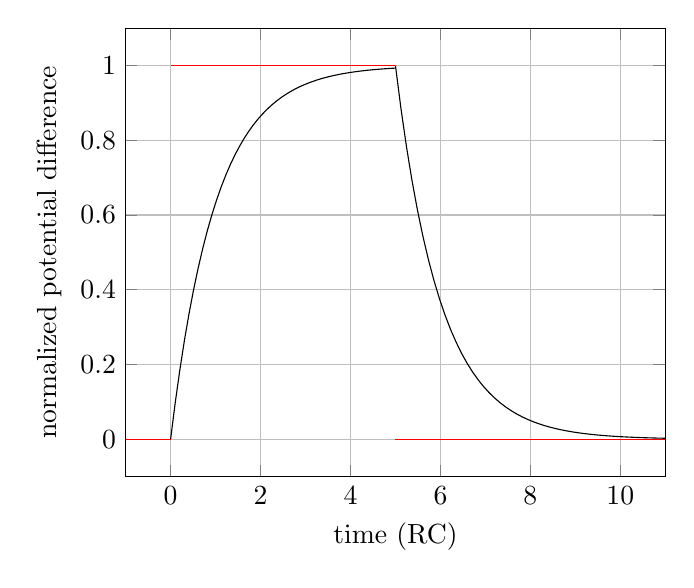
\begin{tikzpicture} 
\begin{axis}[xmin=-1,xmax=11,ymin=-0.1,ymax=1.1,xlabel={time (RC)}, ylabel={normalized potential difference},no markers,samples=50,grid=both]
	\addplot[domain=0:5, black] {1-exp(-x)};
	\addplot[domain=-1:0, red] {0};
	\draw [color=red, dashed] (10,10) -- (10,110);
	\addplot[domain=0:5, red] {1};
	\addplot[domain=5:11, black] {exp(-x+5)};
	\draw [color=red, dashed] (60,10) -- (60,110);
        \addplot[domain=5:11, red] {0};
	\draw [color=red, fill=white] (10,10) circle [radius=0.1cm];
	\draw [color=red, fill=white] (10,110) circle [radius=0.1cm];
	\draw [color=red, fill=red] (10,60) circle [radius=0.1cm];
	\draw [color=red, fill=white] (60,10) circle [radius=0.1cm];
        \draw [color=red, fill=white] (60,110) circle [radius=0.1cm];
        \draw [color=red, fill=red] (60,60) circle [radius=0.1cm];
	\draw [color=black, fill=black] (20,73.2) circle [radius=0.1cm] node[right] {0.632};
	\draw [color=black, fill=black] (40,105) circle [radius=0.1cm] node[below] {0.95};
	\draw [color=black, fill=black] (70,46.8) circle [radius=0.1cm] node[right] {0.368};
	\draw [color=black, fill=black] (90,15) circle [radius=0.1cm] node[above] {0.05};
\end{axis}
\end{tikzpicture}
\caption[Charging and discharging the series $RC$ circuit.]{Charging and discharging the series $RC$ circuit.
Red: normalized input voltage ($V_{in}$) to the series $RC$ circuit, two consecutive \emph{Heaviside step functions}, the second one is inversed and shifted $5RC$ to the right.
Black: normalized output voltage ($V_{out}$) of the series $RC$ circuit.}
\label{fig:charge_discharge}
\end{figure}

To make Eqs. \ref{eq:loop11}-\ref{eq:loop12} useful in electrochemistry, we need to further modify them.
In potentiometry, the important parameter is the potential of the measuring electrode.
We always speak in terms of electrode potential, but it must be born in mind that it is measured with respect to the reference electrode, hence it is always a potential difference.
But since we will take the difference between these differences as well, we just use the expression $potential$ to refer to the state of the potentiometric cell at any time instance $t$.
In the generalized expression we substitute $V_{out}$ for $E_{cell}(t)$, and $V_{in}$ for $E_{cell}(\infty)$.
Also, it is useful to generalize it for changes starting, and ending at any potential value, not just $0$ or $E_{out}$.
After these generalizations, from both equations we get:

\begin{equation}
\label{eq:rc}
        E_{cell}(t) = E_{cell}(\infty) + [E_{cell}(0) - E_{cell}(\infty)]e^{-t/RC}
\end{equation}

This equation \cite{lindner1986definition} will be modified later in the thesis to estimate $E_{cell}(\infty)$ based on the other variables.

\subsection{On the use of the expression ,,equilibrium''}
Throughout my dissertation I use the expression \emph{equilibrium} to describe a steady potential difference between the two terminals of the cell, the electrical contact of the measuring and the reference electrodes.
However, this state of course cannot be regarded an equilibrium, since given enough time, the potential difference will reach zero eventually.
The resistance of the whole cell is finite, and if there is a potential difference between any two points in the cell, current will flow.
Two phenomena have to be distinguished.
The first is the electrochemical process, which is in equilibrium \emph{only} if cell potential difference have reached zero, i.e. the cell is depleted.
The other process is the charging or discharging of a capacitance modeled by $C$ in Fig. \ref{fig:rc}.
This is the total capacitance of the measuring system, including the capacitance of the cables, and the amplifier input as well.
If we accept the model described in the previous section, this can be regarded a purely physical process, which is in true equilibrium if the voltage across the capacitor $C$ is the same as the voltage of the input ($V_i = V_o$). This state is what I refer to by equilibrium.

It must be kept in mind however, that the source of the potential difference in fact \emph{does} change over time for a given electrolyte composition as a consequence of the very small current flowing through the cell (fA range). Therefore it is not an equilibrium, only a steady state.
\newpage
\section{Scanning Electrochemical Microscopy}
\subsection{Origins of the technique}
Scanning Electrochemical Microscopy (SECM) is a branch of the Scanning Probe Microscopic techniques (SPM), of which the first was the Scanning Tunnelling Microscopy (STM), invented by Binnig and Rohrer in 1982 \cite{binnig1982surface} building on their previous studies of controlled vacuum tunnelling published in 1981 \cite{binnig1982physica, binnig1982tunneling}.
They received the Nobel Prize in 1986 \emph{,,for their design of the scanning tunneling microscope''}.
It was a revolutionary technique, the first of its kind, and a pioneer for the other scanning techniques that followed.
STM is capable of incredible resolution, down to the atomic scale.
Optical techniques do not have the resolving power to distinguish details at the atomic level, since they are limited by the wavelength of photons \cite{abbe1873beitrage}.
For instance, wavelength of visible light is in the range of 390 -- 700 nm, while the atomic radii range from 30 pm to 300 pm.
On the other hand, the probes used in STM are extremely sharp, usually just a few atoms at their tip.
There is a potential difference between the tip of the probe and the sample.
As a consequence, a small current will flow between them.
The magnitude of this current depends on the probe -- sample distance.
The image is created by plotting the registered current as a function of the spatial coordinate of each measurement.

The next SPM technique, the Atomic Force Microscopy (AFM), was introduced not long after, in 1986 by Binnig \cite{binnig1986atomic, bennig1988atomic}.
He writes in \cite{binnig1986atomic}:

\begin{quote}
\vspace{0.5cm}
\emph{,,The atomic force microscope is a combination of the principles of the scanning tunneling microscope and the stylus profilometer.
It incorporates a probe that does not damage the surface.
Our preliminary results in air demonstrate a lateral resolution of 30 \AA $ $ and a vertical resolution less than 1  \AA. ...
We envision a general-purpose device that will measure any type of force; not only the interatomic forces, but electromagnetic forces as well.''}
\vspace{0.5cm}
\end{quote}

Indeed, since its invention, AFM has found many applications, and became an invaluable tool of surface analysis.
After these two techniques were established, many more SPM variants followed in a relatively quick succession.
Here a few are mentioned in chronological order:

\begin{itemize}
\item MFM, magnetic force microscopy (1988) \cite{hartmann1988magnetic}
\item SICM, scanning ion-conductance microscopy (1989) \cite{hansma1989scanning}
\item BEEM, ballistic electron emission microscopy (1990) \cite{kaiser1990direct}
\item EFM, electrostatic force microscopy (1991) \cite{weaver1991high}
\item KPFM, kelvin probe force microscopy (1991) \cite{nonnenmacher1991kelvin}
\item SHPM, scanning Hall probe microscopy (1992) \cite{chang1992scanning}
\item SThM, scanning thermal microscopy (1994) \cite{xu1994thermal}
\item SVM, scanning voltage microscopy (1998) \cite{trenkler1998nanopotentiometry}
\end{itemize}

The electrochemical version of SPM, the Scanning Electrochemical Microscope (SECM\footnote{The acronym \emph{,,SECM''} is used for referring to both the technique (Scanning Electrochemical Microscopy) and the instrument itself (Scanning Electrochemical Microscope).}) was introduced in 1989 by Allen J. Bard \cite{bard1989scanning}, \emph{,,the father of modern electrochemistry''}, main author and editor of the monography about SECM \cite{bard1994scanning}\footnote{Recently, a new version of the book has been published \cite{bard2012scanning}.}.
It must be mentioned however, that the notion of spatially resolved chemical information was first proposed by Engstrom, three years earlier, in 1986.
He published a paper about measurements with a microelectrode in the diffusion layer of another electrode, using a bipotentiostat and a micro-manipulator \cite{engstrom1986measurements}.
He writes in 1989 \cite{engstrom1989scanning} referring to his 1986 paper \cite{engstrom1986measurements}:

\begin{quote}
\vspace{0.5cm}
\emph{,,The concept behind what has come to be called SECM was first demonstrated in 1986, when microelectrodes were used to amperometrically detect chemical species produced at a specimen electrode.''}
\vspace{0.5cm}
\end{quote}

But the term \emph{,,Scanning Electrochemical Microscope''} was coined by Allen J. Bard, and he and his coworkers generalized the idea to three dimensions, and layed down the foundations and theory of the technique. 

The two main variants of the technique are the amperometric and the potentiometric modes.
For the first few years, the SECM was only used in amperometric mode.
The next step towards obtaining true chemical information, not just surface topography and conductivity, was the combination of potentiometry and the SECM.
Although several papers have been published already about spatially resolved potentiometric scans, the first potentiometric SECM images appeared on the pages of the paper of Horrocks and Bard written in cooperation with my doctoral supervisor, Professor Géza Nagy \cite{horrocks1993scanning}.
I used very similar antimony microelectrodes as SECM probes to measure local pH throughout my work, and prepared them in the same way as described in that paper. 

\subsection{Potentiometric SECM}
The potentiometric probe is passive, it does not generate or collect, and it can be described as \textbf{\emph{,,substrate generates / substrate collects -- tip detects''}} staying with the original naming scheme.
In this mode, similar to the other modes, the probe is scanned through the points of a raster grid (Fig. \ref{fig:secm}).
But instead of an amperometric measurement, the potential of the probe is measured against a reference electrode, immersed in the same electrolyte at a fixed location.
For the reasons detailed in the section ,,The potentiometric measurement'', a voltage follower is introduced between the electrometer and the measuring electrode.
The first complete work featuring potentiometric SECM images were published in 1993 \cite{horrocks1993scanning}.
In that work, the authors successfully measured pH on a microscale with an antimony microelectrode. 

Later, potentiometric SECM found an application in corrosion science.
Research\-ers in that field are curious about the concentration of certain ions in the electrolyte adjacent of the corroding sample.
Ion-selective electrodes and the SECM are good tools to study the dissolution of these ions.
Concentration profiles of zinc \cite{bastos2010micropotentiometric}, magnesium \cite{lamaka2008monitoring, lamaka2009novel, karavai2010localized} and hydrogen ions \cite{lamaka2008monitoring} were recorded by several research groups.

\begin{figure}[h]
\centering
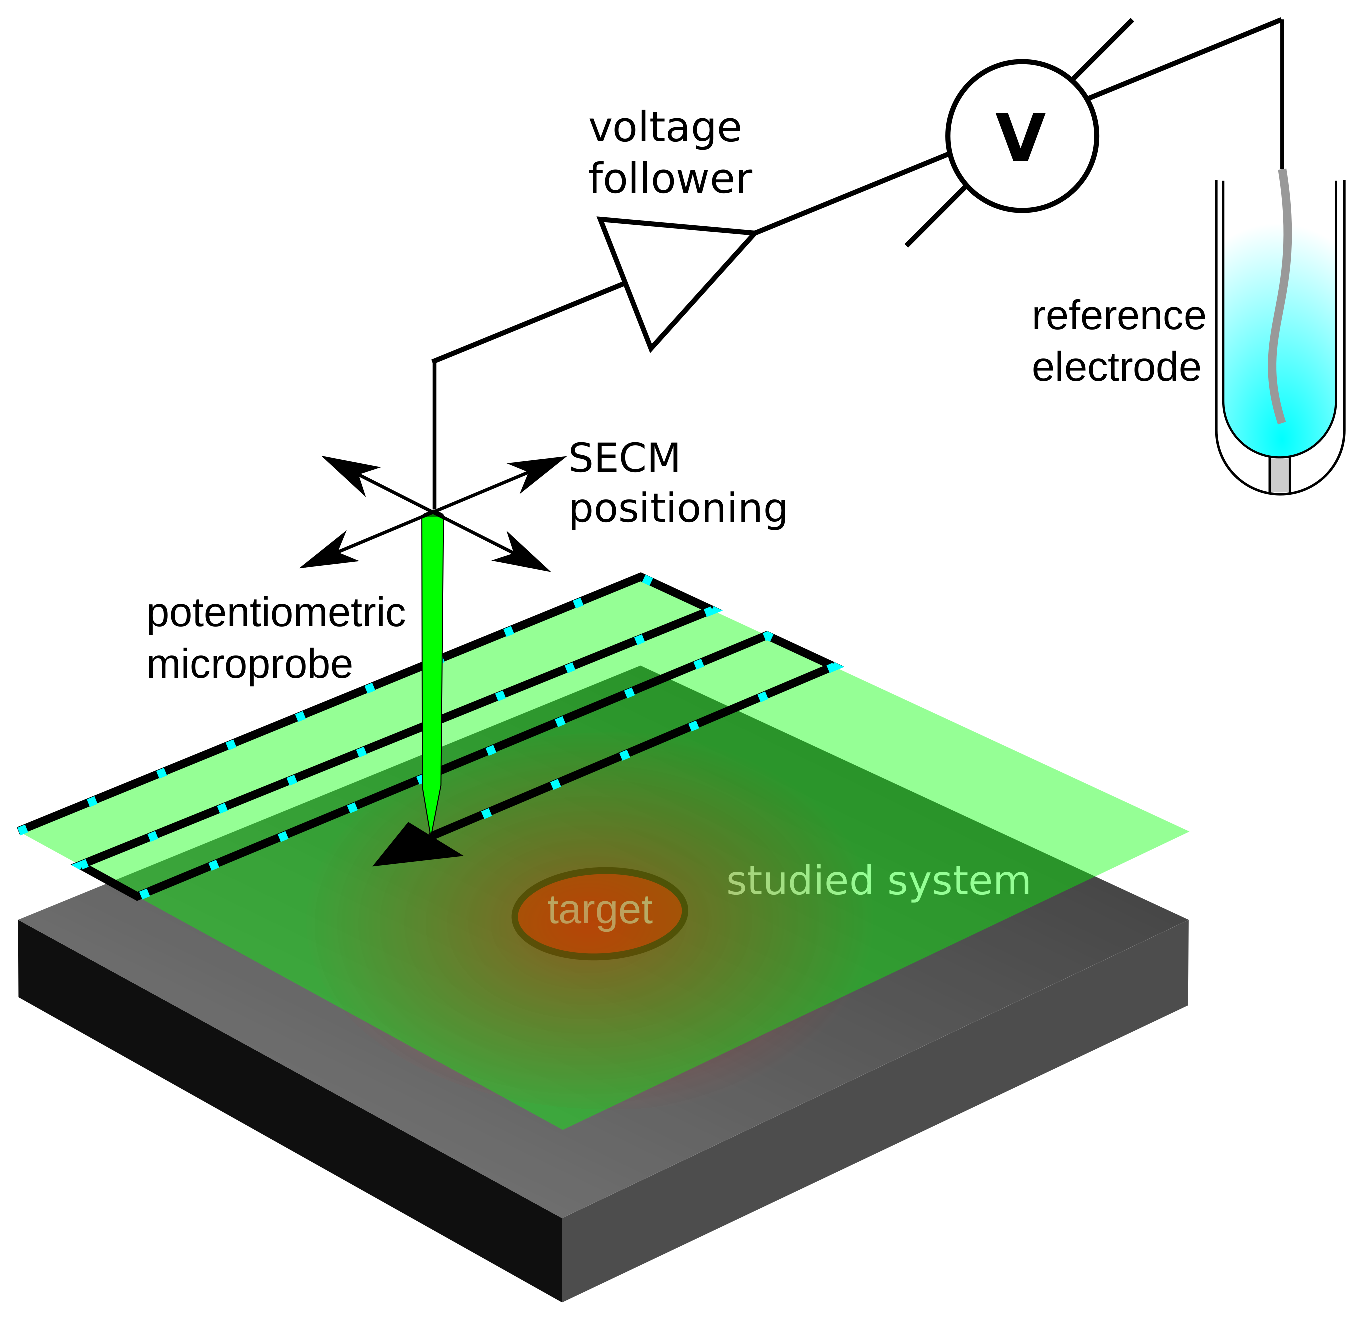
\includegraphics[width=0.6\textwidth]{img/theory/secm.eps}
\caption[A typical potentiometric SECM setup.]{A typical potentiometric SECM setup.
The probe is scanned through the points of a 2D raster at a constant height above the studied surface.
The probe is stopped at every sampling points (here blue dots), and the potential against a reference electrode is recorded.
For potentiometric microelectrodes, the use of a voltage follower is necessary to avoid loading error and reduce noise.}
\label{fig:secm}
\end{figure}

Compared to amperometric SECM studies, the number of papers dealing with potentiometric SECM is relatively low.
I have mentioned the reasons for this in the \emph{,,Motivation''} section

\begin{itemize}
\item It is a lot harded to carry out these kind of experiments,
\item the electrodes are a lot more fragile,
\item Z-axis positioning is more difficult, because most ion-selective microelectrodes cannot double as amperometric probes.
\end{itemize}

There are certain kind of ion-selective microelectrodes, that can be used in both potentiometric, and amperometric mode, although not simultenaously. An example of this type is the antimony/antimony-oxide microelectrode. There are multiple papers featuring this technique, with different kind of electrodes \cite{csoka2009carbon, izquierdo2011novel, filotas2016combined}.

\subsection{Distortion and image processing in SECM}
Signal processing techniques has been widely used in optical microscopy \cite{schrader1996potential}, and in scanning probe microscopy to decrease imaging distortion.
Distortion is any difference between the obtained image and reality.
It is caused by the imperfection of the measuring system, which can be modeled as a measurement transfer function, or convolution function $F$, such that the output $y(t)$ can be written as a function of the input $x$ as

\begin{equation}
\label{convolution}
        y(t) = F(x(t))
\end{equation}

If $F$ is known, the inverse function $F^{-1}$ can be found and used as deconvolution function.

There are many sources of SPM imaging distortion.
In atomic force microscopy, and scanning tunnelling microscopy, it is usually a consequence of the tip-sample interaction, causing the various artefacts \cite{peter2010atomic}.
Broadening of nanometer-scale features by up to three times is a common occurance in STM \cite{lo1993investigation}.
The deconvolution function in this case is closely related to the geometry of the tip and its angle compared to the sample.
If these are known, image restoration is possible by deconvoluting in the spatial domain \cite{chen2006deconvolution, osiro2012measuring, bukharaev1998three}.
Time, and frequency domain deconvolution is also commonly used in SPM techniques to remove time-dependent image artefacts, usually caused by the relatively long response time compared to scanning speed \cite{robinson1988increasing}.


Deconvolution of images obtained with the scanning electrochemical microscope has also been reported by the Bard group \cite{lee1991scanning}.
In that work, amperometric images have been restored (deblurred) by a linear combination of Laplacian and Gaussian filtering.
The main source of distortion in amperometric SECM imaging is the feature broadening caused by diffusion.
The deconvolution function was derived from Fick's law of diffusion, and used as a calculation kernel to cycle through the data points of the 2D raster and obtain the deblurred image.

\begin{figure}
\centering
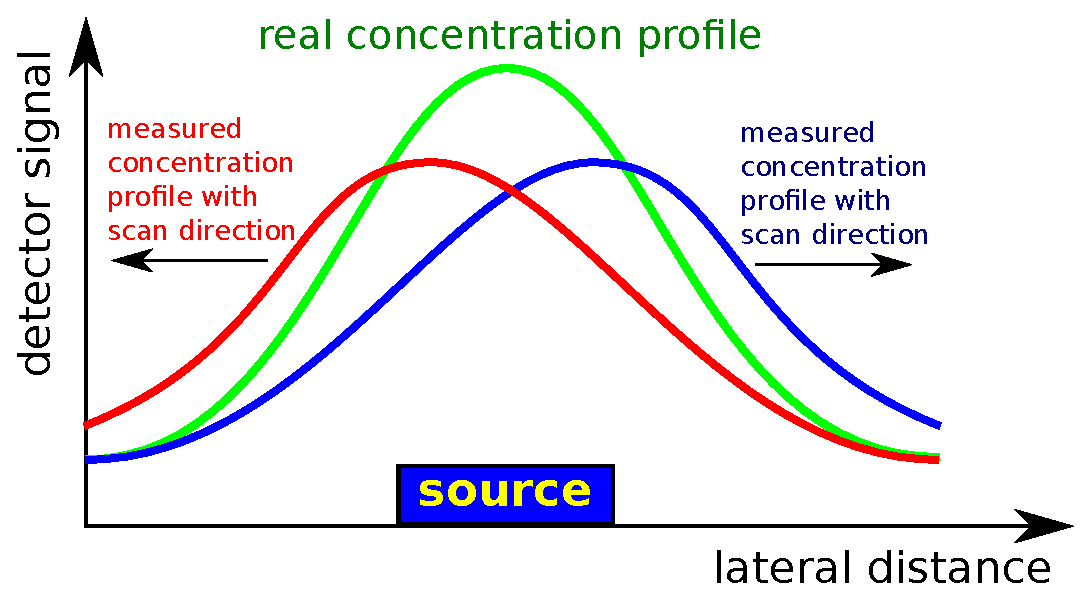
\includegraphics[width=0.6\textwidth]{img/theory/distortion3.eps}
\caption[The distortive effect of potentiometric SECM imaging.]{The distortive effect of potentiometric SECM imaging when scanning at relatively high speed.
The effective speed of the probe is too high, and therefore the time available for the potentiometric cell is too short to reach equilibrium before recording the potential difference at a given point.
The image is blurred along the scan line in the direction of the scan.}
\label{fig:distortion}
\end{figure}
